\chapter{Relatividad General}
\section{Introducción}
Este capítulo es una breve introducción a la teoría de la relatividad general, partiendo desde el concepto de variedad, el espacio tangente y cotangente, el concepto de curvatura y el papel que juega la gravedad en todas estas ideas matemáticas. Las referencias clave de este capítulo son \cite{Carroll,Munkres,bishop_goldberg_1980,wald_2010}.
\section{Variedades}
\subsection{Mapas}
\begin{defi}[Mapa]
	Dados dos conjuntos $A$ y $B$, un mapa $\phi:M\rightarrow N$ es una relación que asigna cada elemento $x\in M$ a un único elemento $y\in N$. En este caso, se denota como $\phi(x)=y$.
\end{defi}
\begin{defi}[Composición de Mapas]
	Con dos mapas $\phi:A\rightarrow B$ y $\Psi:B\rightarrow C$, se define la composición de ambos mapas, $\Psi\circ\phi:A\rightarrow C$, por su acción sobre los elementos de $A$:
	$$(\Psi\circ\phi)(a)=\Psi(\phi(a)).$$
\end{defi}
\begin{center}
	\begin{tikzcd}
		A \arrow[rr, "\Psi\circ\phi"] \arrow[rd, "\phi"] &                      & C \\
		& B \arrow[ru, "\Psi"] &  
	\end{tikzcd}
\end{center}

Un mapa $\phi:A\rightarrow B$ se dice inyectivo (uno a uno) si cada elemento de $B$ tiene a lo sumo un elemento de $A$ que es mapeado a él. Este mapa se dice sobreyectivo si cada elemento de $B$ tiene al menos un elemento de $A$ mapeado a él. $A$ se conoce como el dominio del mapa $\phi$, y su imagen es
$$\mathop{Im}\phi:=\{y\in B: \exists x\in A \text{ tal que }\phi(x)=y\}.$$
La preimagen de un conjunto $U\subseteq B$ bajo la función $\phi$ se define como
$$\phi^{-1}(U):=\{ x\in A: \exists y \in U \text{ tal que }\phi(x)=y\}.$$
Un mapa $\phi:A\rightarrow B$ que es inyectivo y sobreyectivo a la vez se conoce como invertible (biyectivo). En este caso, se define el mapa inverso $\phi^{-1}:B\rightarrow A$ de modo que se satisfaga que, para todo $y\in B$ $(\phi\circ\phi^{-1})(y)=y.$
\begin{center}
	\begin{tikzcd}
		A \arrow[r, "\phi", bend right] & B \arrow[l, "\phi^{-1}"', bend right]
	\end{tikzcd}
\end{center}

Un mapa $f$ de $\mathbb{R}^m$ a $\mathbb{R}^n$ toma una $m-$tupla $(x^1,x^2,\dots,x^m)$ y la envía a una $n-$tupla $(y^1,y^2,\dots,y^n)$, de modo que se puede pensar como una colección de $n$ funciones $\phi^i$ de $m$ variables:
$$y^i=\phi^i(x^1,\dots,x^m)\text{ con }i=1,\dots,n,$$
de modo que
$$f(x^1,\dots,x^m)=(\phi^1(x^1,\dots,x^m),\dots,\phi^n(x^1,\dots,x^m)).$$
Se referirá a cada una de las funciones $\phi^i$ como $C^p$ si son continuas y $p-$veces diferenciables, y al mapa entero $f:\mathbb{R}^m\rightarrow \mathbb{R}^n$ como $C^p$ si cada uno de los campos escalares $\phi^i, i=1,\dots,n$ es al menos $C^p$.

Un mapa $C^0$ es continuo pero no necesariamente diferenciable, mientras que un mapa $C^\infty$ es continuo y puede ser diferenciado cuantas veces se desee. Los mapas $C^\infty$ se llaman suaves.
\begin{defi}[Difeomorfismo]
	El mapa $\phi:A\rightarrow B$ se conoce como difeomorfismo si es biyectivo, y tanto él como su inversa son $C^\infty$. Se dice entonces que los conjuntos $A$ y $B$ son difeomorfos.
\end{defi}

\subsection{Regla de la cadena}
Si tiene dos mapas $f:\mathbb{R}^m\rightarrow \mathbb{R}^n$ y $g:\mathbb{R}^n\rightarrow\mathbb{R}^l,$ que se componen en $(g\circ f):\mathbb{R}^m\rightarrow\mathbb{R}^l$, represente cada espacio en términos de coordenadas: $x^a$ en $\mathbb{R}^m$, $y^b$ en $\mathbb{R}^n$ y $z^c$ en $\mathbb{R}^l$, donde los índices $a,b,c$ varían sobre los valores apropiados.
\begin{center}
	\begin{tikzcd}
		\mathbb{R}^m \arrow[rd, "f"] \arrow[rr, "g\circ f"] &                              & \mathbb{R}^l \\
		& \mathbb{R}^n \arrow[ru, "g"] &             
	\end{tikzcd}
\end{center}

La regla de la cadena relaciona las derivadas parciales de la composición $(g\circ f)$ con las derivadas parciales de los mapas $f$ y $g$ de la siguiente manera
$$\frac{\partial}{\partial x^a}(g\circ f)^c=\sum_{b=1}^n\frac{\partial f^b}{\partial x^a}\frac{\partial g^c}{\partial y^b}.$$

\subsection{Variedades}
En el capítulo de estabilidad se trató el concepto de variedad como un espacio métrico homeomorfo localmente a la bola abierta. En este capítulo se tomará una variedad más general: la variedad topológica, para lo cual se introducirá la idea de topología, y demás conceptos necesarios en términos de la topología de la variedad.
\begin{defi}[Espacio topologico]
	Tome $A$ como un conjunto arbitrario. $\tau$ es una topología para el conjunto $A$ si satisface las siguientes condiciones:
	\begin{enumerate}
		\item $\emptyset,A\in\tau$,
		\item Si $\{U_\alpha\}_{\alpha\in I}\subset\tau$ es una familia arbitraria de elementos de $\tau$, entonces la unión de toda esta familia pertenece a $\tau$, es decir, $\bigcup_{\alpha\in I} U_\alpha\in\tau$, y
		\item Si $\{U_n\}_{n=1}^m\subset\tau$ es una familia finita de elementos de $\tau$, entonces la intersección de todos sus elementos también es un elemento de $\tau,$ es decir, $\bigcap_{n=1}^m U_n\in\tau$.
	\end{enumerate}
	En este caso se dice que la pareja $(A,\tau)$ es un espacio topológico. Los elementos de $\tau$ se llaman abiertos y sus complementos se llaman cerrados.
\end{defi}
\begin{defi}[Carta o sistema coordenado]
	Considere un espacio topológico $(M,\tau)$. Una carta o sistema coordenado $(U, \phi)$ consiste de un conjunto abierto $U\subset M$, junto con un mapa inyectivo $\phi:U\rightarrow\mathbb{R}^n,$ tal que $\phi(U)$ es abierto en $(\mathbb{R}^n, \tau_u)$\footnote{$\tau_u$ denota la topología usual sobre $\mathbb{R}^n$.}.
\end{defi}
\begin{defi}[Atlas $C^r$]
	Un atlas $C^r$ es una colección indexada de cartas $\{(U_\alpha.\phi_\alpha)\}_{\alpha\in I}$, con $\phi_\alpha$ siendo al menos $C^r$, para todo $\alpha\in I$, que satisface las siguientes condiciones
	\begin{enumerate}
		\item $\bigcup_{\alpha\in I} U_\alpha=M$, es decir, $\{U_\alpha\}_{\alpha\in I}$ es un cubrimiento abierto para $M$ y
		\item si para algunos $\alpha,\beta\in I$ ($\alpha\neq\beta$), $U_\alpha\cap U_\beta\neq\emptyset$, entonces el mapa $(\phi_\alpha\circ\phi_\beta^{-1}):\phi_\beta(U_\alpha\cap U_\beta)\rightarrow\phi_\alpha(U_\alpha\cap U_\beta)$ toma puntos en $\phi_\beta(U_\alpha\cap U_\beta)\subseteq\mathbb{R}^n$ y los envía a puntos en $\phi_\alpha(U_\alpha\cap U_\beta)$, y viceversa. Ambas composiciones deben ser $C^r$. Si se satisface esta condición se dice que los mapas $\phi_\alpha$ y $\phi_\beta$ son compatibles
	\end{enumerate}
	
	Un atlas se dice maximal si contiene todas las posibles cartas compatibles.
\end{defi}
\begin{center}
	\begin{tikzcd}
		U_\alpha\cap U_\beta\subset M \arrow[d, "\phi_\beta"] \arrow[rr, "\phi_\alpha"]                    &  & \phi_\alpha(U_\alpha\cap U_\beta)\subset\mathbb{R}^n \arrow[lld, "\phi_\beta\circ\phi_\alpha^{-1}", bend left] \\
		\phi_\beta(U_\alpha\cap U_\beta)\subset\mathbb{R}^n \arrow[rru, "\phi_\alpha\circ\phi_\beta^{-1}"] &  &                                                                                                               
	\end{tikzcd}
\end{center}
\begin{defi}[$C^r$ Variedad $n-$dimensional]
	Una $C^r$ variedad $n-$dimensional es un espacio topológico $(M,\tau)$ junto con un atlas maximal $C^r$.
\end{defi}
El hecho de que una variedad sea localmente como $\mathbb{R}^n$ (a través de las cartas) introduce la posibilidad de usar herramientas del cálculo real sobre ella. Tome por ejemplo dos $C^\infty$ variedades $(M,\tau_M)$ y $(N,\tau_N)$ de dimensión $m$ y $n$, respectivamente. Por simplicidad, pero sin pérdida de generalidad, tome $\phi:M\rightarrow\mathbb{R}^m$ y $\Psi:N\rightarrow\mathbb{R}^n$ como las cartas coordenadas de $M$ y $N$, respectivamente. Si $f:M\rightarrow N$ es una función entre ambas variedades,

\begin{center}
	\begin{tikzcd}
		M \arrow[rr, "f"]                                                            &  & N \arrow[d, "\Psi"] \\
		\mathbb{R}^m \arrow[rr, "\Psi\circ f \circ\phi^{-1}"] \arrow[u, "\phi^{-1}"] &  & \mathbb{R}^n       
	\end{tikzcd}
\end{center}
se puede introducir el concepto de diferenciación sobre el mapa $f$, construyendo el mapa
$$(\Psi\circ f\circ \phi^{-1}):\mathbb{R}^m\rightarrow\mathbb{R}^n,$$
de modo que el operador $\frac{\partial f}{\partial x^\mu}$ quede definido como
$$\frac{\partial f}{\partial x^\mu}:=\frac{\partial }{\partial x^\mu}(\Psi\circ f\circ \phi^{-1}),$$
donde $\mu=1,\dots,m$.
\subsection{Espacio tangente y cotangente}
Tome $\mathcal{F}$ como el espacio de todas las funciones suaves $f:M\rightarrow\mathbb{R}$ ($\phi^{-1}\circ f$ es de clase $C^\infty$, siendo $\phi$ la carta coordenada de $M$). Cada curva $\gamma:\mathbb{R}\rightarrow M$ que pasa por algún punto $p\in M$ define un operador sobre el espacio, la derivada direccional, que mapea $f$ a $$\frac{\mathrm{d}f}{d\lambda}\Big|_{\lambda: \gamma(\lambda)=p}:=\frac{\mathrm{d}}{d\lambda}(f\circ\gamma)(\lambda)$$ (evaluada en $p$).
\begin{center}
	\begin{tikzcd}
		\mathbb{R} \arrow[r, "\gamma"] \arrow[rr, "f\circ\gamma"', bend right] & M \arrow[r, "f"] & \mathbb{R}
	\end{tikzcd}
\end{center}
\begin{defi}[Espacio tangente]
	El espacio tangente $T_pM$ a un punto $p\in M$ es el espacio de los operadores derivadas direccionales dados por todas las curvas que pasan por el punto $p$. Este espacio resulta ser un espacio vectorial.
\end{defi}
El espacio tangente $T_pM$ posee una base natural, $\{\partial_\mu\}$. Cada uno de estos operadores está definido en términos de la curva generada por la carta coordenada del punto $p$. Es decir, si $(U,\phi)$ es una carta coordenada tal que $p\in U$, se toma $(\phi^{-1})^\mu:\mathbb{R}\rightarrow M$ como la restricción de la función $\phi^{-1}$ a una única variable, $x^\mu$, $\mu=1,\dots,m$, con el objetivo de que esta nueva función sea una curva sobre $M$ que pase por $p$, para que defina la derivada direccional $\partial_\mu.$

Para ver que efectivamente es una base del espacio tangente $T_pM$, considere una variedad $m$-dimensional suave $M$, una carta coordenada $(U,\phi)$, una curva $\gamma:\mathbb{R}\rightarrow M$ y una función $f: M\rightarrow \mathbb{R}$.

\begin{center}
	\begin{tikzcd}
		\mathbb{R} \arrow[rrdd, "\phi\circ\gamma"'] \arrow[rr, "\gamma"] \arrow[rrrr, "f\circ\gamma", bend left] &  & U\subseteq M \arrow[dd, "\phi"', bend right] \arrow[rr, "f"]                       &  & \mathbb{R} \\
		&  &                                                                                    &  &            \\
		&  & \mathbb{R}^m \arrow[uu, "\phi^{-1}"', bend right] \arrow[rruu, "f\circ\phi^{-1}"'] &  &           
	\end{tikzcd}
\end{center}
Si $\lambda$ es el parámetro de la curva $\gamma$, se expande el operador $\frac{\mathrm{d}}{\mathrm{d}\lambda}$ en términos de los operadores $\partial_\mu$ aplicando la regla de la cadena:
$$\frac{\mathrm{d}f}{\mathrm{d}\lambda}=\frac{\mathrm{d}}{\mathrm{d}\lambda}(f\circ\gamma)=\frac{\mathrm{d}}{\mathrm{d}\lambda}((f\circ\phi^{-1})\circ(\phi\circ\gamma))=\frac{\mathrm{d}(\phi\circ\gamma)^\mu}{\mathrm{d}\lambda}\frac{\partial(f\circ\phi^{-1})}{\partial x^\mu}=\frac{\mathrm{d}x^\mu}{\mathrm{d}\lambda}\partial_\mu f.$$
Como la función $f$ es arbitraria,
$$\frac{\mathrm{d}}{\mathrm{d}\lambda}=\frac{\mathrm{d}x^\mu}{\mathrm{d}\lambda}\partial_\mu,$$
con lo que los operadores derivada direccional $\{\partial_\mu\}$ son una base para $T_pM$, conocida como base coordenada. Además, esto implica que el espacio tangente $T_pM$ tiene la misma dimensión de la variedad.

Una de las ventajas de este punto de vista de los vectores como operadores diferenciales es que la ley de transformación es inmediata. Como los vectores de la base son $\hat{e}_{(\mu)}=\partial_{\mu}$, los vectores de la base en un nuevo sistema coordenado $x^{\mu'}$ están dadas por la regla de la cadena \cite{Carroll}

$$\partial_{\mu^{\prime}}=\frac{\partial x^{\mu}}{\partial x^{\mu^{\prime}}} \partial_{\mu}$$

La ley de transformación de vectores se introduce de tal forma que un vector del espacio tangente $V=V^\mu \partial_\mu$ permanezca invariante bajo un cambio de base, es decir,
$$V^\mu\partial_\mu=V^{\mu'}\partial_{\mu'}=V^{\mu'}\frac{\partial x^\mu}{\partial x^{\mu'}}\partial_\mu,$$
y como la matriz $\frac{\partial x^{\mu'}}{\partial x^{\mu}}$ es la inversa de $\frac{\partial x^\mu}{\partial x^{\mu'}}$, la ley de transformación es

\begin{equation}
	V^{\mu'}=\frac{\partial x^{\mu'}}{\partial x^{\mu}} V^\mu.
\end{equation}
\begin{defi}[Espacio cotangente]
	El espacio cotangente $T^*_pM$ de una variedad $M$ en un punto $p\in M$ es el conjunto de los mapas lineales $\omega:T_pM\rightarrow \mathbb{R}$. Los elementos de este espacio se conocen como 1-formas.
\end{defi}

El ejemplo canónico de 1-forma es el gradiente de una función $f:M\rightarrow \mathbb{R}$, denotado por $\mathrm{d}f$. Su acción sobre un vector $\frac{\mathrm{d}}{\mathrm{d}\lambda}$ del espacio tangente es exactamente la derivada direccional sobre la función $f$:
$$\mathrm{d}f\left( \frac{\mathrm{d}}{\mathrm{d}\lambda} \right)=\frac{\mathrm{d}f}{\mathrm{d}\lambda}\Big|_{p}.$$
Justo como las derivadas parciales a lo largo de los ejes coordenados proveen una base natural para el espacio tangente, los gradientes de las funciones coordenadas $x^\mu$ proveen una base natural para el espacio cotangente $\{\mathrm{d}x^\mu\}$, conocida como base dual. Observe que, al aplicar $\mathrm{d}x^\mu$ a $\partial_\eta$ se obtiene que
$$\mathrm{d}x^\mu(\partial_\nu)=\frac{\partial x^\mu}{\partial x^\nu}=\frac{\partial}{\partial x^\nu}(x^\mu\circ (x^\nu)^{-1})=\frac{\partial}{\partial x^\nu}((x^\mu\circ\phi^{-1})\circ(\phi\circ (x^\nu)^{-1})).$$
\begin{center}
\begin{tikzcd}
\mathbb{R} \arrow[rr, "(x^\nu)^{-1}"] \arrow[rrdd, "\phi\circ(x^\nu)^{-1}"'] &  & M \arrow[dd, "\phi"]                                                      &  &                       \\
                                                                             &  &                                                                           &  &                       \\
                                                                             &  & \mathbb{R}^m \arrow[rr, "\phi^{-1}"] \arrow[rrdd, "x^\mu\circ\phi^{-1}"'] &  & M \arrow[dd, "x^\mu"] \\
                                                                             &  &                                                                           &  &                       \\
                                                                             &  &                                                                           &  & \mathbb{R}           
\end{tikzcd}
\end{center}

Aplicando la regla de la cadena,
$$\frac{\partial}{\partial x^\nu}((x^\mu\circ\phi^{-1})\circ(\phi\circ (x^\nu)^{-1}))=\frac{\partial(\phi\circ(x^\nu)^{-1})^\eta}{\partial x^\nu}\frac{\partial(x^\mu\circ\phi^{-1})}{\partial x^\eta}.$$
Intuitivamente, $x^\mu\circ\phi^{-1}=x^\mu,$ donde $x^\mu$ del lado izquierdo de la igualdad es la $\mu$-ésima coordenada de la carta, y al lado derecho es la $\mu$-ésima componente de $\mathbb{R}^m$. Por otro lado, $(\phi\circ(x^\nu)^{-1})^\eta=x^\eta,$ con lo que
$$\frac{\partial(\phi\circ(x^\nu)^{-1})^\eta}{\partial x^\nu}\frac{\partial(x^\mu\circ\phi^{-1})}{\partial x^\eta}=\frac{\partial x^\eta}{\partial x^\nu}\frac{\partial x^\mu}{\partial x^\eta}=\delta_\eta^\mu \frac{\partial x^\eta}{\partial x^\nu}=\frac{\partial x^\mu}{\partial x^\nu}=\delta_\nu^\mu.$$
En resumen,
\begin{equation}
	\boxed{\mathrm{d}x^\mu(\partial_\nu)=\delta_\nu^\mu.}
\end{equation}
Esta condición determina que $\{\mathrm{d}x^\mu\}$ es una base para el espacio cotangente $T^*_p M$ \cite{Carroll}. De este modo, cualquier 1-forma $\omega$ se puede expandir en sus componentes: $\omega=\omega_\mu \mathrm{d}x^\mu$. Las propiedades de transformación de los vectores de la base dual y las componentes de una 1-forma se siguen de la misma forma que en el caso del espacio tangente:
$$\mathrm{d}x^{\mu'}=\frac{\partial x^{\mu'}}{\partial x^\mu} \mathrm{d}x^\mu;\ \omega_{\mu'}=\frac{\partial x^\mu}{\partial x^{\mu'}}\omega_\mu.$$

\begin{defi}[Espacio producto cartesiano]
	Se define el espacio producto cartesiano $\Pi_l^k$ respecto a un punto $p\in M$ de la variedad como:
	$$\Pi_l^k:=\underbrace{T^*_pM\times\cdots\times T^*_pM}_{l-\text{veces}}\times \underbrace{T_pM\times\cdots\times T_pM}_{k-\text{veces}}, \text{ es decir,}$$
	$$\Pi_l^k=\{(\omega^1,\omega^2,\dots,\omega^l,\mathds{X}_1,\mathds{X}_2,\dots,\mathds{X}_k): \omega^i\in T^*_pM; \ \mathds{X}_i\in T_pM\}.$$
	Este espacio es un espacio vectorial con la suma y el producto usuales.
\end{defi}
\begin{defi}[Tensores]
	Un tensor $(k,l)$ $\mathds{T}:\Pi_l^k\rightarrow \mathbb{R}$ es un mapa multilineal (lineal en cada uno de sus argumentos). Este tensor se puede expandir en términos de las bases del espacio tangente y cotangente de la siguiente forma:
	
	$$\mathds{T}=?{T}^{\mu_1\cdots\mu_k}_{\nu_1\cdots{\nu_l}}? \partial_{\mu_1}\otimes \cdots\otimes \partial_{\mu_k}\otimes \mathrm{d}x^{\nu_1}\otimes\cdots\otimes \mathrm{d}x^{\nu_l},$$
	donde $?{T}^{\mu_1\cdots\mu_k}_{\nu_1\cdots{\nu_l}}?$ son los coeficientes del tensor.
\end{defi}
De modo similar al caso de los vectores, los tensores transforman coordenadas en cada uno de sus índices de la siguiente forma:
$$?T^{\mu_1'\cdots\mu_k'}_{\nu_1'\cdots\nu_l'}?=\frac{\partial x^{\mu_1'}}{\partial x^{\mu_1}}\cdots\frac{\partial x^{\mu_k'}}{\partial x^{\mu_k}}\frac{\partial x^{\nu_1}}{\partial x^{\nu_1'}}\cdots \frac{\partial x^{\nu_l}}{\partial x^{\nu_l'}}?{T}^{\mu_1\cdots\mu_k}_{\nu_1\cdots{\nu_l}}?.$$
Infortunadamente, la derivada parcial de un tensor no es, en general, un tensor (no cumple esta regla de transformación de coordenadas). Esto motivará posteriormente la derivada covariante, que preservará el carácter tensorial tras aplicarse sobre un tensor.

\begin{defi}[Tensor métrico]
	El tensor métrico $?g_{\mu\nu}?$ es un tensor simétrico $(0,2)$, cuya representación matricial tiene determinante no nulo ($g=|g_{\mu\nu}|\neq0$), y satisface la relación
	\begin{equation}\label{metricTensor}
		?g^{\mu\nu}? ?g_{\nu\sigma}?= ?\delta^\mu_\sigma?.
	\end{equation}
	La simetría de $?g_{\mu\nu}?$ implica la simetría de $?g^{\mu\nu}?$, y la relación \eqref{metricTensor} permite que el tensor métrico se pueda usar para subir o bajar índices.
\end{defi}
\begin{defi}[Elemento de línea]
	El elemento de línea se define de la siguiente forma
	$$\mathrm{d}s^2=?g_{\mu\nu}? \mathrm{d}x^\mu \mathrm{d}x^\nu.$$
\end{defi}
\section{Curvatura}
\subsection{Derivada covariante}
Como se comentó en la sección anterior, es necesario definir un operador derivada (denotado por $\nabla$), que lleve a cabo las operaciones de la derivada parcial usual, pero de manera independiente de las coordenadas, y que a su vez preserve el carácter tensorial tras ser aplicada a un tensor. $\nabla$ debe ser un mapa de los tensores $(k,l)$ a los tensores $(k.l+1)$ que guarda las siguientes propiedades
\begin{enumerate}
	\item Linealidad: $\nabla(T+S)=\nabla T+\nabla S$.
	\item Ley del producto de Leibniz: $\nabla(T\otimes S)=(\nabla T)\otimes S+T\otimes(\nabla S).$
\end{enumerate}
Si $\nabla$ obedece la regla de la cadena, $\nabla$ se puede escribir como una derivada parcial más alguna transformación lineal \cite{Thorne}. Entonces, se toma primero la derivada parcial y se aplica una corrección lineal para hacer el resultado covariante. Se propone entonces, para un vector del espacio tangente:
\begin{equation}
\nabla_\mu V^\nu= \partial_\mu V^\nu+?\Gamma^\nu_{\mu\lambda}? V^\lambda,
\end{equation}
donde $?\Gamma^\nu_{\mu\lambda}?$ son las componentes de la matriz (no es un tensor, porque no transforma como tal) que se encarga de realizar la corrección. Todas estas componentes reciben el nombre de símbolos de Christoffel.

De modo similar al caso del vector del espacio tangente, la derivada covariante de una 1-forma se puede expresar como una derivada parcial más alguna transformación lineal:
$$\nabla_\mu \omega_\nu=\partial_\mu \omega_\nu+ ?\Xi^\lambda_{\mu\nu}?\omega_\lambda,$$
donde $?\Xi^\lambda_{\mu\nu}?$ podría ser distinta, en general, de $?\Gamma^\lambda_{\mu\nu}?$. Se exigen además las siguientes propiedades para la derivada covariante:

\begin{enumerate}
	\setcounter{enumi}{2}
	\item Conmutación bajo contracciones: $\nabla_\mu(?T^\lambda_{\lambda\rho}?)=(\nabla T?)_\mu^\lambda_{\lambda\rho}?$.
	\item Se reduce a la derivada parcial en el caso de escalares: $\nabla_\mu\phi=\partial_\mu\phi.$
\end{enumerate}
No hay forma de derivar estas propiedades, simplemente se exige que sean ciertas \cite{Carroll}. A continuación se verán las implicaciones de estas propiedades. Si $\omega_\mu$ es una 1-forma y $V^mu$ es un vector, se puede tomar la derivada covariante del escalar definido por $\omega_\lambda V^\lambda$, obteniendo
\begin{dmath}\label{equivGamma}
	\nabla_\mu(\omega_\lambda V^\lambda) = (\nabla_\mu \omega_\lambda)V^\lambda+\omega_\lambda( \nabla_\mu V^\lambda) = (\partial_\mu \omega_\lambda + ?\Xi^\sigma_{\mu\lambda}?\omega_\sigma)V^\lambda+\omega_\lambda(\partial_\mu V^\lambda+?\Gamma^\lambda_{\mu\sigma}? V^\sigma) = (\partial_\mu \omega_\lambda)V^\lambda+?\Xi^\sigma_{\mu\lambda}? \omega_\sigma V^\lambda + \omega_\lambda(\partial_\mu V^\lambda)+\omega_\lambda ?\Gamma^\lambda_{\mu\sigma} V^\sigma?. 
\end{dmath}
Por otro lado, como $\omega_\lambda V^\lambda$ es un escalar,
\begin{equation}\label{equivGamma2}
	\nabla_\mu(\omega_\lambda V^\lambda)=\partial_\mu(\omega_\lambda V^\lambda)=(\partial_\mu\omega_\lambda) V^\lambda+\omega_\lambda(\partial_\mu V^\lambda).
\end{equation}
Igualando \eqref{equivGamma} y \eqref{equivGamma2}, se obtiene que
$$?\Xi^\sigma_{\mu\lambda}?=-?\Gamma^\sigma_{\mu\lambda}?.$$ 
De esta forma, el resultado tras aplicar la derivada covariante sobre una 1-forma es
\begin{equation}
	\nabla_\mu \omega_\nu=\partial_\mu \omega_\nu- ?\Gamma^\lambda_{\mu\nu}?\omega_\lambda.
\end{equation}
La generalización para un tensor $(k,l)$ es
\begin{dmath}
	\nabla_\sigma ?T^{\mu_1\cdots\mu_k}_{\nu_1\cdots\nu_l}?=\partial_\sigma ?T^{\mu_1\cdots\mu_k}_{\nu_1\cdots\nu_l}?+?\Gamma^{\mu_1}_{\sigma\lambda}??T^{\lambda\cdots\mu_k}_{\nu_1\cdots\nu_l}?+\cdots+?\Gamma^{\mu_k}_{\sigma\lambda}??T^{\mu_1\cdots\lambda}_{\nu_1\cdots\nu_l}?-?\Gamma^\lambda_{\sigma\nu_1}??T^{\mu_1\cdots\mu_k}_{\lambda\cdots\nu_l}?-\cdots-?\Gamma^\lambda_{\sigma\nu_l}??T^{\mu_1\cdots\mu_k}_{\nu_1\cdots\lambda}?.
\end{dmath}
Generalmente se abrevia la derivada covariante de la siguiente manera:
$$\nabla_\sigma ?T^{\mu_1\cdots\mu_k}_{\nu_1\cdots\nu_l}?=?T^{\mu_1\cdots\mu_k}_{\nu_1\cdots\nu_l;\sigma}?.$$
Par construir esta derivada covariante es necesario agregar una conexión a la variedad, que transforme de tal forma que anule los términos que impiden la transformación tensorial de la derivada parcial usual. 

En lo que refiere a la unicidad, se garantiza si se suponen las siguientes condiciones:
\begin{itemize}
	\item libre de torsión: $?\Gamma^\lambda_{\mu\nu}?=?\Gamma^\lambda_{(\mu\nu)}?$ (la conexión es simétrica) y
	\item compatibilidad con la métrica: $\nabla_\rho ?g_{\mu\nu}?=0.$
\end{itemize}
Para demostrar este hecho, considere las tres permutaciones posibles de la compatibilidad con la métrica.
\begin{equation}\label{compa1}
\nabla_\rho ?g_{\mu\nu}? =\partial_\rho?g_{\mu\nu}?-?\Gamma^\lambda_{\rho\mu}? ?g_{\lambda\nu}?-?\Gamma^\lambda_{\rho\nu}? ?g_{\mu\lambda}?=0,
\end{equation}
\begin{equation}\label{compa2}
\nabla_\mu ?g_{\nu\rho}? =\partial_\mu?g_{\nu\rho}?-?\Gamma^\lambda_{\mu\nu}? ?g_{\lambda\rho}?-?\Gamma^\lambda_{\mu\rho}? ?g_{\nu\lambda}?=0,
\end{equation}
\begin{equation}\label{compa3}
\nabla_\nu ?g_{\rho\mu}? =\partial_\nu?g_{\rho\mu}?-?\Gamma^\lambda_{\nu\rho}? ?g_{\lambda\mu}?-?\Gamma^\lambda_{\nu\mu}? ?g_{\rho\lambda}?=0.
\end{equation}
Realizando la operación \eqref{compa1}-\eqref{compa2}-\eqref{compa3}, y aplicando la simetría de la conexión, se obtiene lo siguiente
$$\partial_\rho ?g_{\mu\nu}?-\partial_\mu ?g_{\nu\rho}?-\partial_\nu ?g_{\rho\mu}?+2 ?\Gamma^\lambda_{\mu\nu}? ?g_{\lambda\rho}?=0,$$
de modo que al despejar $?\Gamma^\lambda_{\mu\nu}?$ con la ayuda de la métrica inversa $?g^{\sigma\rho}?$ se tiene que

\begin{equation}\label{conectionChristoffel}
?\Gamma^\sigma_{\mu\nu}?=\frac{1}{2}?g^{\sigma\rho}?[\partial_\mu ?g_{\nu\rho}?+\partial_\nu ?g_{\rho\mu}?-\partial_\rho ?g_{\mu\nu}?].
\end{equation}
Esta última fórmula prueba tanto la existencia como la unicidad y se conoce como conexión de Christoffel, conexión de Levi-Civita o conexión Riemanniana. Los coeficientes de conexión se conocen como símbolos de Christoffel.

Una manera de escribir la contracción $?\Gamma^\mu_{\mu\lambda}?$ de los símbolos de Christoffel se basa en la siguiente propiedad que cumple cualquier matriz $M$ \cite{bishop_goldberg_1980}
$$\mathop{Tr}(M^{-1}\partial_\lambda M)=\partial_\lambda \mathop{ln} \mathop{det} M,$$
con la cual
\begin{equation}
?\Gamma^\mu_{\mu\lambda}?=\frac{1}{\sqrt{|g|}}\partial_\lambda\sqrt{|g|},
\end{equation}
donde $|g|=\mathop{det}g.$ Con esta forma de escribir $?\Gamma^\mu_{\mu\lambda}?$, se tiene que cualquier derivada covariante de un vector $V^\mu$ se puede reescribir de la siguiente forma
\begin{equation}
\nabla_\mu V^\mu=\frac{1}{\sqrt{|g|}}\partial_\mu(\sqrt{|g|}V^\mu).
\end{equation}

\subsection{Transporte paralelo}
Un concepto recurrente en el espacio plano es el transporte paralelo, que busca mantener un vector (tensor) constante conforme uno se mueve a través de una trayectoria. Dada una curva $x^\mu(\lambda)$, el requerimiento de la constancia de un tensor $T$ a lo largo de la curva en el espacio plano es $$\frac{\mathrm{d}T}{\mathrm{d}\lambda}=\frac{\mathrm{d}x^\mu}{\mathrm{d}\lambda}\frac{\partial T}{\partial x^\mu}=0.$$ De este modo, en analogía con el caso planar, se define la derivada covariante a lo largo de una trayectoria $x(\lambda)$  sobre la variedad como el operador
\begin{equation}
\frac{\mathrm{D}}{\mathrm{D}\lambda}\equiv \frac{\mathrm{d}x^\mu}{\mathrm{d}\lambda}\nabla_\mu.
\end{equation}
Con ello, se define el transporte paralelo del tensor $T$ a lo largo de la trayectoria $x(\lambda)$ bajo el requerimiento de que, a lo largo de dicha trayectoria:
\begin{equation}\label{3.31}
\left(\frac{\mathrm{D}T}{\mathrm{D}\lambda}\right)\indices{^{\mu_1\cdots\mu_k}_{\nu_1\cdots\nu_\ell}}\equiv \frac{\mathrm{d}x^\sigma}{\mathrm{d}\lambda}\nabla_\sigma T\indices{^{\mu_1\cdots\mu_k}_{\nu_1\cdots\nu_\ell}}=0.
\end{equation}
Esta última ecuación recibe el nombre de \textbf{ecuación de transporte paralelo}. Para un vector $V^\mu$ toma la forma
\begin{equation}
	\frac{\mathrm{d}V^\mu}{\mathrm{d}\lambda}+\Gamma\indices{^\mu_{\sigma\rho}}\frac{\mathrm{d}x^\sigma}{\mathrm{d}\lambda}V^\rho=0.
\end{equation}
Se puede ver la ecuación de transporte paralelo como una ecuación diferencial de primer orden que define un problema de valor inicial: dado un tensor en algún punto del camino, hay una única continuación del tensor a otros puntos a través del camino tal que la continuación satisface \eqref{3.31}. Se dice entonces que el tensor es transportado paralelamente.

Por supuesto, la noción de transporte paralelo depende de la conexión, por lo que diferentes conexiones llevan a distintas soluciones. Si la conexión es compatible con la métrica:
$$\frac{\mathrm{D}g_{\mu\nu}}{\mathrm{D}\lambda}=\frac{\mathrm{d}x^\sigma}{\mathrm{d}\lambda}\nabla_\sigma g_{\mu\nu}=0,$$
lo que implica que la métrica es transportada paralelamente. Una propiedad interesante que satisface una métrica transportada paralelamente es que el producto interno dos vectores paralelamente transportados es preservado a lo largo de la trayectoria. Esto es, si $V^\mu$ y $W^\mu$ son dos vectores paralelamente transportados, se tiene que
$$\frac{\mathrm{D}}{\mathrm{D}\lambda}\left( g_{\mu\nu}V^\mu W^\nu\right)=\left(\frac{\mathrm{D}}{\mathrm{D}\lambda}g_{\mu\nu}\right)V^\mu W^\nu+g_{\mu\nu}\left(\frac{\mathrm{D}}{\mathrm{D}\lambda}V^\mu\right)W^\nu+g_{\mu\nu}V^\mu \left(\frac{\mathrm{D}}{\mathrm{D}\lambda}W^\nu\right)=0,$$
de donde se deduce que el transporte paralelo con respecto a una conexión compatible con la métrica preserva la norma de vectores.

Se define ahora una \textbf{geodésica} como una trayectoria que transporta paralelamente su propio vector tangente. El vector tangente a una trayectoria $x(\lambda)$ es $\frac{\mathrm{d}x^\mu}{\mathrm{d}\lambda}$, de modo que la condición de transporte paralelo para este vector es
\begin{equation}
\frac{\mathrm{D}}{\mathrm{D}\lambda}\frac{\mathrm{d}x^\mu}{\mathrm{d}\lambda}=0,
\end{equation}
o de manera alternativa,
\begin{equation}\label{geodesicEquation}
	\frac{\mathrm{d}^2x^\mu}{\mathrm{d}\lambda^2}+\Gamma\indices{^\mu_{\rho\sigma}}\frac{\mathrm{d}x^\rho}{\mathrm{d}\lambda}\frac{\mathrm{d}x^\sigma}{\mathrm{d}\lambda}=0.
\end{equation}
Esta última expresión recibe el nombre de \textbf{ecuación de la geodésica}. También se puede obtener esta expresión a través de un principio variacional sobre la acción $\sqrt{-g_{\mu\nu}\frac{\mathrm{d}x^\mu}{\mathrm{d}\lambda}\frac{\mathrm{d}x^\nu}{\mathrm{d}\lambda}}$, para trayectorias tipo tiempo \cite{Carroll}.

\subsection{Tensor de Riemann}
La curvatura se cuantifica mediante el tensor de Riemann, que se deriva de la conexión. La idea detrás de la medición de la curvatura es que se tiene una idea natural de planitud de la conexión: la conexión de Christoffel convencional asociada a la métrica Minkowskiana o euclideana tiene varias propiedades que se pueden ver como manifestaciones de planitud. Algunas de ellas son las siguientes:
\begin{itemize}
	\item El transporte paralelo alrededor de una trayectoria cerrada deja el vector invariante.
	\item Las derivadas covariantes de tensores conmutan.
	\item Las geodésicas que inician paralelas siguen siendo paralelas.
\end{itemize}
El tensor de Riemann surge cuando se estudia cómo cambian estas propiedades en contextos más generales. Una manera convencional de introducir el tensor de Riemann es considerar transportes paralelos alrededor de un loop infinitesimal. Imagine que se transporta paralelamente un vector $V^\sigma$ alrededor de un loop cerrado definido por dos vectores $A^\nu$ y $B^\mu$ (ver figura \ref{fig:loops}). Como se sabe que la acción del transporte paralelo es independiente de las coordenadas, debe haber algún tensor que diga cómo cambia el vector cuando vuelve a su punto inicial.

\begin{figure}
\begin{center}
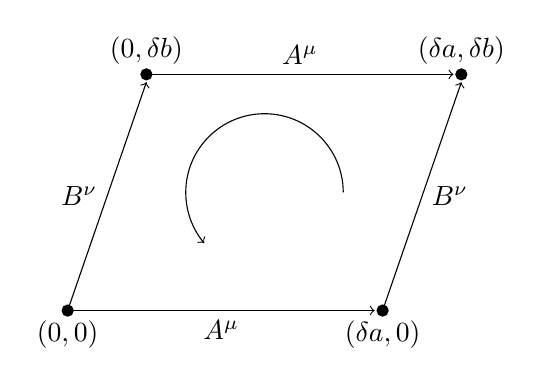
\begin{tikzpicture}
\filldraw [black] (0,0) circle (2pt) node[below] {$(0,0)$};
\filldraw [black] (1,3.) circle (2pt) node[above] {$(0,\delta b)$};
\filldraw [black] (5,3.) circle (2pt) node[above] {$(\delta a,\delta b)$};
\filldraw [black] (4,0) circle (2pt) node[below] {$(\delta a,0)$};
\draw[->] (3.5,1.5) arc (0:220:1);
\draw[->] (0,0) -- (1,2.9) node[midway, left] {$B^\nu$};
\draw[->] (1,3) -- (4.9,3) node[midway, above] {$A^\mu$};
\draw[->] (0,0) -- (3.9,0) node[midway, below] {$A^\mu$};
\draw[->] (4,0) -- (5,2.9) node[midway, right] {$B^\nu$};
\end{tikzpicture}
\end{center}

\caption{Esquema de transporte paralelo del vector $V^\sigma$ alrededor de un loop cerrado definido por los vectores $A^\nu$ y $B^\mu$, y las longitudes infinitesimales de los lados del loop son $\delta a$ y $\delta b$.}
\label{fig:loops}
\end{figure}

Se tendrá entonces una transformación lineal sobre el vector, de modo que el tensor encargado de esta corrección tendrá un índice superior y otro inferior. Por otro lado, este tensor dependerá de los vectores $A$ y $B$ que determinan el loop, por lo que tendrá otros dos índices inferiores adicionales para contraer $A^\nu$ y $B^\mu$. Más aún, el tensor debe ser antisimétrico en estos dos índices, porque intercambiarlos corresponde a recorrer el loop al revés. Se espera entonces que la expresión para el cambio $\delta V^\rho$ experimentado por este vector cuando es transportado paralelamente por el loop sea de la forma \cite{Carroll}
\begin{equation}\label{alternativeRiemann}
	\delta V^\rho\equiv (\delta a)(\delta b)A^\nu B^\mu R\indices{^\rho_{\sigma\mu\nu}}V^\rho,
\end{equation}
donde $R\indices{^\rho_{\sigma\mu\nu}}$ es un tensor $(1,3)$ conocido como \textbf{tensor de Riemann} (o tensor de curvatura), antisimétrico en sus dos últimos índices:
$$R\indices{^\rho_{\sigma\mu\nu}}=-R\indices{^\rho_{\sigma\nu\mu}}.$$
Para encontrar $R\indices{^\rho_{\sigma\mu\nu}}$ en términos de los coeficientes de la conexión, se usa la conmutación de las derivadas covariantes, que mide la diferencia entre el transporte paralelo de un tensor a través de una curva infinitesimal y luego a través de otra, contra el orden opuesto.

\begin{figure}
\begin{center}
\begin{tikzpicture}
\filldraw [black] (0,0) circle (2pt);
\filldraw [black] (1,3.) circle (2pt);
\filldraw [black] (5,3.) circle (2pt);
\filldraw [black] (4,0) circle (2pt);

\draw[->] (0,0) -- (1,2.9) node[midway, left] {$\nabla_\nu$};
\draw[->] (1,3) -- (4.9,3) node[midway, above] {$\nabla_\mu$};
\draw[->] (0,0) -- (3.9,0) node[midway, below] {$\nabla_\mu$};
\draw[->] (4,0) -- (5,2.9) node[midway, right] {$\nabla_\nu$};
\end{tikzpicture}
\end{center}

\caption{Conmutación de las derivadas covariantes.}
\label{fig:CovariantLoops}
\end{figure}
Así, si calcula el conmutador de las derivadas covariantes $[\nabla_\mu,\nabla_\nu]$, aplicado sobre un vector $V^\rho$, se obtiene que
\begin{dmath}
[\nabla_\mu,\nabla_\nu]V^\rho=\left(\partial_\mu \Gamma\indices{^\rho_{\nu\sigma}}-\partial_\nu \Gamma\indices{^\rho_{\mu\sigma}}+\Gamma\indices{^\rho_{\mu\lambda}}\Gamma\indices{^\lambda_{\nu\sigma}}-\Gamma\indices{^\rho_{\nu\lambda}}\Gamma\indices{^\lambda_{\mu\sigma}}\right)V^\sigma -\left(\Gamma\indices{^\lambda_{\mu\nu}}-\Gamma\indices{^\lambda_{\mu\sigma}}\right)\left(\partial_\lambda V^\rho+\Gamma\indices{^\rho_{\lambda\sigma}} V^\sigma\right) = \left(\partial_\mu \Gamma\indices{^\rho_{\nu\sigma}}-\partial_\nu \Gamma\indices{^\rho_{\mu\sigma}}+\Gamma\indices{^\rho_{\mu\lambda}}\Gamma\indices{^\lambda_{\nu\sigma}}-\Gamma\indices{^\rho_{\nu\lambda}}\Gamma\indices{^\lambda_{\mu\sigma}}\right)V^\sigma -2\Gamma\indices{^\lambda_{[\mu\nu]}}\nabla_\lambda V^\rho.
\end{dmath}
De este modo, se reescribe el conmutador como
\begin{equation}
[\nabla_\mu,\nabla_\nu]=R\indices{^\rho_{\sigma\mu\nu}}-T\indices{^\lambda_{\mu\nu}}\nabla_\lambda,
\end{equation}
donde $T\indices{^\lambda_{\mu\nu}}$ es la antisimetrización sobre los índices inferiores de los símbolos de Christoffel, y se identifica el tensor de Riemann con
\begin{equation}\label{riemannDefinition}
R\indices{^\rho_{\sigma\mu\nu}}=\partial_\mu \Gamma\indices{^\rho_{\nu\sigma}}-\partial_\nu \Gamma\indices{^\rho_{\mu\sigma}}+\Gamma\indices{^\rho_{\mu\lambda}}\Gamma\indices{^\lambda_{\nu\sigma}}-\Gamma\indices{^\rho_{\nu\lambda}}\Gamma\indices{^\lambda_{\mu\sigma}}.
\end{equation}
Se puede demostrar que la definición del tensor de Riemann dada en \eqref{alternativeRiemann} es equivalente a \eqref{riemannDefinition} \cite{wald_2010}. Por otro lado, este tensor es efectivamente un tensor, a pesar de estar conformado de elementos que no son tensores.

Algunas ecuaciones importantes que satisface el tensor de Riemann son las siguientes,
\begin{equation}\label{susceptibilityContracted}
\nabla_\lambda R_{\rho\sigma\mu\mu}+\nabla_\rho R_{\sigma\lambda\mu\nu}+\nabla_\sigma R_{\lambda\rho\mu\nu}=0,
\end{equation}
\begin{equation}
\nabla_{[\lambda}R_{\rho\sigma]\mu\nu}=0.
\end{equation}
Esta última ecuación se conoce como identidad de Bianchi. Por otro lado, algunas contracciones importantes del tensor de Riemann son el tensor de Ricci
\begin{equation}\label{ricciTensor}
	R_{\mu\nu}=R\indices{^\lambda_{\mu\lambda\nu}},
\end{equation}
que resulta ser simétrico; y el escalar de Ricci

\begin{equation}\label{ricciScalar}
	R=R\indices{^\mu_\mu}=g^{\mu\nu}R_{\mu\nu}.
\end{equation}
Una expresión especialmente útil se obtiene al contraer dos veces \eqref{susceptibilityContracted}.

\begin{dmath*}
0=g^{\nu\sigma}g^{\mu\lambda}\left(\nabla_\lambda R_{\rho\sigma\mu\mu}+\nabla_\rho R_{\sigma\lambda\mu\nu}+\nabla_\sigma R_{\lambda\rho\mu\nu}\right) = g^{\nu\sigma}\left(\nabla^\mu R_{\rho\sigma\mu\nu-\nabla_\rho} R\indices{^\mu_{\sigma\mu\nu}}+\nabla_\sigma R\indices{^\mu_{\rho\mu\nu}}\right) = -\nabla^\mu\left( R\indices{^\nu_{\rho\mu\nu}}\right)-\nabla_\rho R+\nabla^nu R_{\rho\nu} = \nabla^\mu R_{\rho\mu}-\nabla_\rho R+\nabla^\nu R_{\rho\nu}.
\end{dmath*}
En el desarrollo anterior se usó la compatibilidad con la métrica para introducirla dentro de las derivadas covariantes, para subir y bajar índices. De este modo,
\begin{equation}\label{interest}
\frac{1}{2}\nabla_\rho R=\nabla^\mu R_{\rho\mu}.
\end{equation}
Si se define el tensor de Einstein (simétrico) como 
\begin{equation}
	G_{\mu\nu}=R_{\mu\nu}-\frac{1}{2}Rg_{\mu\nu},
\end{equation}
es claro por \eqref{interest} que
\begin{equation}
	\nabla^\mu G_{\mu\nu}=0.
\end{equation}
\section{Gravitación}
Los postulados fundamentales de la relatividad son los siguientes:
	\begin{enumerate}
		\item En presencia de gravedad, el espacio-tiempo luce como una variedad curvada 4-dimensional (con componentes del tensor de Riemann en general no nulas).
		\item No hay forma de distinguir la aceleración uniforme de un campo gravitacional externo.
		\item Las partículas libres se mueven a lo largo de geodésicas.
	\end{enumerate}  
Se define ahora el límite Newtoniano por los siguientes tres requerimientos: las partículas se mueven lentamente (con respecto a la velocidad de la luz), el campo gravitacional es plano (puede considerarse como una perturbación del espacio plano) y el campo gravitacional es estático (no varía en el tiempo). Tomando el tiempo propio $\tau$ como parámetro afín, la ecuación de la geodésica \eqref{geodesicEquation} es
\begin{equation}
\frac{\mathrm{d}^2x^\mu}{\mathrm{d}\tau^2}+\Gamma\indices{^\mu_{\rho\sigma}}\frac{\mathrm{d}x^\rho}{\mathrm{d}\tau}\frac{\mathrm{d}x^\sigma}{\mathrm{d}\tau}=0.
\end{equation}
Moverse lentamente implica que la partícula avanza más en el tiempo que en el espacio. Matemáticamente, esta condición se escribe como
\begin{equation}
	\frac{\mathrm{d} x^{i}}{\mathrm{d}\tau}<<\frac{\mathrm{d} t}{\mathrm{d}\tau},
\end{equation}
donde $i=1,2,3.$ De este modo, la ecuación de la geodésica queda escrita como
\begin{equation}\label{geodesicNewtonian}
\frac{\mathrm{d}^2x^\mu}{\mathrm{d}\tau^2}+\Gamma\indices{^\mu_{00}}\left(\frac{\mathrm{d}t}{\mathrm{d}\tau}\right)^2=0.
\end{equation}
Ahora, los símbolos de Christoffel de la forma $\Gamma\indices{^\mu_{00}}$ son, usando \eqref{conectionChristoffel}, y teniendo en cuenta que el campo es estático:
$$\Gamma\indices{^\mu_{00}}=\frac{1}{2}g^{\mu\lambda}\left( \partial_0 g_{\lambda0}+\partial_0 g_{0\lambda}-\partial_\lambda g_{00}\right)=-\frac{1}{2}g^{\mu\lambda}\partial_\lambda g_{00}.$$
Finalmente, como el campo gravitacional es débil, se puede descomponer la métrica en dos componentes: la métrica de Minkowski $\eta_{\mu\nu}=\mathop{diag}(-1,0,0,0)$ más una perturbación $h_{\mu\nu},$ de modo que
$$g_{\mu\nu}=\eta_{\mu\nu}+h_{\mu\nu}.$$
A primer orden de $h$, se puede usar la métrica de Minkowski para subir y bajar índices. Así,
\begin{equation}
	\Gamma\indices{^\mu_{00}}=-\frac{1}{2}\eta^{\mu\lambda}\partial_\lambda h_{00}.
\end{equation}
La ecuación geodésica \eqref{geodesicNewtonian} es entonces
\begin{equation}
\frac{\mathrm{d}^2x^\mu}{\mathrm{d}\tau^2}=\frac{1}{2}g^{\mu\lambda}\partial_{\lambda}h_{00} \left( \frac{\mathrm{d} t}{\mathrm{d} \tau}\right)^2.
\end{equation}
Como el campo es estático, $\partial_0 h_{00}=0,$ y la componente $\mu=0$ de esta ecuación es
$$\frac{\mathrm{d}^2 t}{\mathrm{d}\tau^2}=0,$$
lo que implica que $\frac{\mathrm{d} t}{\mathrm{d} \tau}$ es una constante. Respecto a las componentes espaciales $i=1,2,3,$
\begin{equation}
\frac{\mathrm{d}^2x^i}{\mathrm{d}\tau^2}=\frac{1}{2}\left( \frac{\mathrm{d} t}{\mathrm{d} \tau}\right)^2 \partial_{i}h_{00}. 
\end{equation}
Dividiendo la última ecuación por $\left( \frac{\mathrm{d} t}{\mathrm{d} \tau}\right)^2$ y aplicando la regla de la cadena, se tiene que
\begin{equation}\label{gravLaw}
	\frac{\mathrm{d}^2x^i}{\mathrm{d}t^2}=\frac{1}{2} \partial_i h_{00}.
\end{equation}
Tomando la componente $h_{00}$ como $-2V(x^i)$ en \eqref{gravLaw}, se obtiene la ley de gravitación universal de Newton. En otras palabras,
\begin{equation}\label{g00}
	\boxed{g_{00}=-\left(1+2V(x^i)\right).}
\end{equation}
Entonces, la curvatura del espacio-tiempo es suficiente para describir el comportamiento de la gravedad en el límite Newtoniano, siempre que la métrica satisfaga \eqref{g00}. La manera de conocer $g_{\mu\nu}$ es mediante las ecuaciones de campo para la métrica, conocidas como ecuaciones de campo de Einstein. Estas ecuaciones se deducen a través de un principio variacional sobre la acción de Hilbert-Einstein
\begin{equation}
	S_H=\int \mathrm{d}^4x\sqrt{-g}\left(R-2\Lambda\right),
\end{equation}
donde $\Lambda$ es la constante cosmológica. De esta forma, las ecuaciones de campo de Einstein son
\begin{equation}\label{fieldEquations}
	R_{\mu\nu}-\frac{1}{2}Rg_{\mu\nu}+\Lambda g_{\mu\nu}=8\pi G T_{\mu\nu},
\end{equation}
donde $T_{\mu\nu}$ es el tensor de momento-energía. De este modo, conociendo la métrica que soluciona \eqref{fieldEquations}, se puede determinar el potencial en el límite Newtoniano (de campo débil), producto de dicha métrica a través de \eqref{g00}. 